\documentclass[conference]{IEEEtran}
\usepackage[utf8]{inputenc}
\usepackage{graphicx}
\usepackage{amsmath}
\usepackage{url}
\usepackage{booktabs}
\usepackage[spanish]{babel}
\usepackage{graphicx}
\usepackage{float}
\usepackage{pdflscape}
\usepackage{listings}
\usepackage{titlesec}
\setlength{\parskip}{0.5em}
\setlength{\parindent}{0pt}


\title{Dinámicas Sociales y Moralidad Colectiva en Reddit: Un Estudio del Subreddit r/AmITheA**hole utilizando técnicas de Machine Learning}

\author{
    \IEEEauthorblockN{
        Carlos Andres Espitia Alfonso\IEEEauthorrefmark{1}, 
        Michael Santiago Moreno Bravo\IEEEauthorrefmark{1},\\
        Juan David Salguero Medina\IEEEauthorrefmark{2}, 
        Juan Diego Yepes Parra\IEEEauthorrefmark{3}
    }
    \IEEEauthorblockA{
        \IEEEauthorrefmark{1}Doctorado en Ingeniería\\
        \IEEEauthorrefmark{2}Pregrado en Ingeniería de Sistemas y Computación,\\
        \IEEEauthorrefmark{3}Maestría en Ingeniería de Sistemas y Computación,\\
        Facultad de Ingeniería, Universidad de los Andes, Bogotá, Colombia
    }
    
}


\begin{document}

\maketitle

\begin{abstract}
    Este trabajo presenta un estudio comparativo de técnicas de aprendizaje automático para la clasificación automática de juicios morales colectivos en el subreddit r/AmITheA**hole (AITA). La comunidad AITA constituye un laboratorio natural donde usuarios solicitan veredictos éticos sobre situaciones personales, generando un dataset único de 30,830 publicaciones con etiquetas morales (YTA, NTA, ESH, NAH, INFO) extraídas de comentarios comunitarios. Se evaluaron sistemáticamente modelos clásicos (SVM, regresión logística, Naive Bayes), arquitecturas de aprendizaje profundo (GRU, BERT, RoBERTa) y grandes modelos de lenguaje (LLaMA 3.1, GPT-4o) en esta tarea de clasificación multiclase con severo desbalance. Los resultados demuestran que los modelos transformer con fine-tuning (BERT, RoBERTa) alcanzan el mejor rendimiento general con accuracy de hasta 74\% y F1-score macro de 0.26, superando significativamente a enfoques clásicos y LLMs sin entrenamiento específico. Sin embargo, todos los modelos enfrentan limitaciones críticas en la detección de clases minoritarias (ESH, NAH, INFO), obteniendo F1-scores nulos. El análisis exploratorio revela patrones temáticos dominantes relacionados con conflictos familiares y de pareja, mientras que experimentos de temperatura en LLMs sugieren que configuraciones deterministas mejoran la consistencia clasificatoria. Este estudio contribuye con una evaluación comprehensiva de paradigmas de IA aplicados al razonamiento moral automatizado, evidenciando tanto el potencial como las limitaciones actuales para modelar juicios éticos colectivos en entornos digitales.
\end{abstract}

\begin{IEEEkeywords}
Moralidad colectiva; Reddit; procesamiento de lenguaje natural; aprendizaje automático; veredictos éticos; clasificación multiclase.
\end{IEEEkeywords}

% Introducción: Justifique el problema abordado, su relevancia y contexto.
\section{Introducción}

Las redes sociales han revolucionado la manera en que las personas interactúan, comparten opiniones y construyen comunidades. Reddit es de las redes sociales más particulares. Especialmente conocida por su estructura y sus foros especializados en los que los usuarios pueden debatir sobre cualquier tema, de forma anónima. Un aspecto interesante de Reddit son sus "subreddits", foros o comunidades centradas en un tema donde los usuarios pueden crear y compartir publicaciones, comentarlas y votar en ellas. 

Dentro de estas comunidades, existe r/AmITheA**hole (AITA), un espacio donde los usuarios comparten historias personales sobre situaciones complejas y piden a la comunidad que los juzgue o aconseje, respondiendo a la pregunta: "¿Soy el a**hole (el malo de la historia)?". Este tipo de interacción genera una fuente de datos o dataset único que puede servir de insumo para uno o varios modelos de aprendizaje automático. Estos datos permiten analizar las dinámicas sociales en línea, la forma en como se toma una decisión colectiva y si es posible automatizarla, y qué factores influyen en la aceptación o rechazo de una historia. 

Esta comunidad ha ganado una popularidad considerable; las publicaciones varían en complejidad, desde simples malentendidos hasta situaciones más serias que involucran relaciones familiares, parejas, amigos o compañeros de trabajo. Los participantes, al presentar sus historias, esperan obtener un veredicto, en la cual se tienen en cuenta los comentarios de la publicación, donde los participantes de la comunidad opinan utilizando un comentario con el voto específico, el cual puede ser YTA you’re the a**hole (eres es el malo), NTA not the a**hole (no eres el malo), ESH everyone sucks here (todos son malos) entre otros votos posibles, al igual que expresan sus opiniones respecto a la situación y los actores.

Existen varios problemas que afectan la calidad del contenido y la carga de trabajo de los moderadores de la comunidad. A medida que la comunidad crece, los moderadores pueden verse sobrecargados con la gestión de las publicaciones, lo cual consume mucho tiempo, especialmente si se alcanza una cantidad significativa de publicaciones diarias. Esta saturación no solo afecta la efectividad de los moderadores, sino que también puede influir en la calidad de las interacciones y en la precisión de los veredictos que se emiten.

Esto abre la posibilidad para considerar una herramienta automatizada que apoye a los moderadores a poner el veredicto en la publicación. La inclusión de dicha herramienta sería en complemento a su labor actual, donde el análisis de publicaciones se puede realizar de manera más eficiente, permitiendo que los moderadores se enfoquen en aspectos más subjetivos y delicados, mientras que el sistema se encargaría de dar una sugerencia de acuerdo al contenido de la publicación.

Por otro lado, se considera de interés investigar los temas que más frecuentemente influencian los veredictos, como las relaciones familiares o las disputas laborales, para poder identificar patrones en la toma de decisiones y en las dinámicas que subyacen a los votos. ¿Por qué algunas historias reciben más popularidad que otras? ¿Es el contenido de las publicaciones lo que determina su aceptación o el perfil del usuario que las comparte? ¿Qué tan relevantes son la longitud del texto y otros factores en la popularidad de un post? Estas preguntas requieren una investigación para entender cómo el algoritmo de Reddit y la interacción humana juegan un papel crucial en los resultados finales.

r/AmITheA**hole ofrece una oportunidad para comprender mejor las dinámicas sociales en línea, así como para investigar cómo se toman decisiones colectivas en estas comunidades. Este conjunto de datos es lo suficientemente grande y diverso como para permitir un análisis profundo de los factores que influyen en la popularidad de las publicaciones y en los veredictos que emiten los usuarios. La variedad de temas tratados en las publicaciones hace que este análisis sea aún más relevante, ya que abarca una gama amplia de situaciones personales y sociales.

Además, este análisis es un ejercicio académico interesante, ya que permite aplicar técnicas de procesamiento de lenguaje natural (NLP) y modelos de machine learning para examinar cómo los usuarios interactúan en este tipo de plataformas. Combinar ambos enfoques ofrece una oportunidad para probar la efectividad de los modelos de manera práctica, obteniendo resultados que puedan contribuir al aprendizaje sobre el funcionamiento de estos sistemas. Finalmente, este ejercicio también puede llegar a ser interesante en la evaluación de modelos extensos de lenguaje (LLMs), utilizando como prompt el post y preguntándole cuál veredicto daría, con el fin de probar programáticamente qué tan acertados son.


\subsection{Objetivo General}
Diseñar, implementar y evaluar un sistema interactivo que integre un conjunto de modelos de aprendizaje automático y técnicas de procesamiento de lenguaje natural (NLP), capaz de analizar publicaciones del subreddit r/AmITheA**hole y predecir de forma automatizada el juicio moral colectivo (etiqueta).

\subsection{Objetivos Específicos}

\begin{itemize}
    \item Desplegar una herramienta que exponga los resultados de los modelos, de forma que sean fáciles de ver.
    \item Encontrar patrones, tendencias, distribuciones y demás insights sobre los datos de las publicaciones de la comunidad.
    \item Probar la efectividad comparativa de diferentes arquitecturas de modelos de lenguaje, desde modelos de machine learning clásico ligeros hasta redes neuronales densas y LLMs, en tareas de clasificación moral en entornos reales.
\end{itemize}

% Trabajos Relacionados (Related Work): Revise literatura y proyectos previos similares, destacando enfoques, resultados y limitaciones.
\section{Trabajos relacionados}

El análisis automatizado de decisiones morales en comunidades en línea, especialmente en Reddit, ha captado la atención académica por su potencial para mejorar la comprensión de las dinámicas sociales en estas plataformas. En particular, investigaciones recientes se han enfocado en estudiar cómo las comunidades virtuales realizan juicios éticos sobre situaciones personales complejas, buscando identificar factores que influyen en el veredicto colectivo, tales como características del contenido, perfil del usuario o señales sociales implícitas.

Botzer \textit{et al.} \cite{botzer2023} abordaron este tema mediante un análisis detallado del subreddit r/AmITheA**hole (AITA), examinando la influencia del género, la edad y el tipo de juicio moral expresado sobre la popularidad y recepción social de las publicaciones. Sus hallazgos mostraron que las historias consideradas moralmente positivas suelen tener mayor aceptación y popularidad, reflejada en una mayor cantidad de votos positivos y comentarios generados por la comunidad. Este estudio utilizó modelos avanzados basados en BERT (Judge-BERT) para clasificar publicaciones según el juicio moral colectivo, destacando la importancia de considerar tanto factores lingüísticos como sociales en la dinámica de aceptación del contenido. Aunque su investigación contribuye significativamente a identificar qué factores influyen en la popularidad de las publicaciones, no considera directamente la automatización de veredictos como herramienta práctica para apoyar a los moderadores, aspecto central en nuestra propuesta.

Por otro lado, Alhassan \textit{et al.} \cite{alhassan2022} presentaron una investigación centrada exclusivamente en la predicción del juicio moral en AITA utilizando modelos avanzados de procesamiento de lenguaje natural (RoBERTa y Longformer). Sus resultados demostraron una alta efectividad (hasta 87\% de precisión), confirmando que estos modelos pueden replicar de forma acertada las decisiones colectivas tomadas por la comunidad. Esta investigación es relevante para nuestro trabajo, ya que valida la aplicación de modelos avanzados para clasificar juicios morales en textos de interacciones cotidianas en línea. Sin embargo, no profundizan en otros aspectos claves que abordaremos, como la influencia de la longitud del texto y otros factores contextuales en la aceptación general de las publicaciones.

Osama y Bsher \cite{osama2023} introdujeron una perspectiva diferente al investigar la generación automática de comentarios con razonamiento moral explícito mediante transformers como BART y T5. Este enfoque mostró que es posible producir contenido automatizado moralmente fundamentado con resultados convincentes desde el punto de vista humano. Aunque nuestro proyecto no contempla la generación de comentarios, este trabajo resalta la complejidad de captar matices éticos mediante técnicas avanzadas de NLP, enfatizando la necesidad de entender profundamente las señales implícitas y explícitas presentes en el contenido generado por los usuarios.

Strathern \textit{et al.} \cite{strathern2020} aportan una perspectiva complementaria al estudiar cómo surgen las 'explosiones de indignación moral' en Twitter. Su estudio analizó 21 casos de indignación colectiva, desarrollando métodos para detectar sistemáticamente estos cambios mediante señales lingüísticas. Los autores encontraron patrones significativos, como la disminución en el uso del pronombre ``yo'' y el incremento de negatividad durante estos episodios. Utilizando técnicas de detección de puntos de cambio, lograron identificar el inicio de estas explosiones aproximadamente media hora antes de su manifestación evidente, demostrando que los cambios en el uso del lenguaje en comentarios textuales pueden proporcionar información sobre el comportamiento cambiante y la perspectiva cambiante.

Preniqi \textit{et al.} \cite{preniqi2024} desarrollaron MoralBERT, un modelo de lenguaje especializado para capturar valores morales en discursos sociales basado en la Teoría de los Fundamentos Morales. Utilizando datasets heterogéneos de Twitter, Reddit y Facebook, implementaron tanto entrenamiento agregado como adversarial de dominio para mejorar la generalización entre plataformas. Sus resultados mostraron que el marco propuesto logra una puntuación F1 promedio entre 11\% y 32\% más alta que enfoques tradicionales, y particularmente relevante para nuestro trabajo es su hallazgo de que modelos especializados de tamaño moderado pueden competir con LLMs gigantes para detectar valores morales, sugiriendo que un enfoque similar podría ser efectivo para la clasificación automática de veredictos en AITA sin requerir recursos computacionales excesivos.


% Metodología: Describa detalladamente el enfoque propuesto, desde la recolección y tratamiento de datos, arquitectura del modelo, entrenamiento, hasta las métricas de evaluación utilizadas.
\section{Metodología}

El diagrama \ref{fig:metodologia} muestra el flujo de la metodología realizada para el proyecto. Esta forma de trabajo está inspirada en la forma en la que se estructuran en su gran mayoría los proyectos de aprendizaje automático, sin tener en cuenta re-entrenamiento u otros aspectos de tener un modelo en productivo a lo largo del tiempo.

\begin{figure}
    \centering
    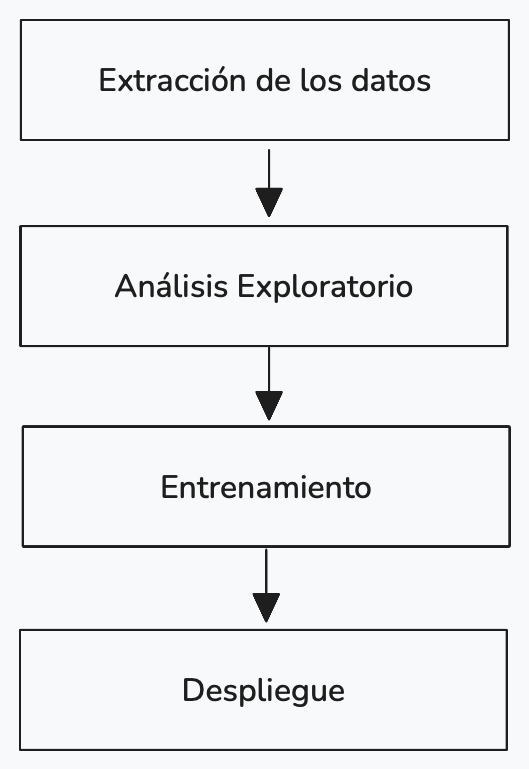
\includegraphics[width=0.2\textwidth]{resources/metodologia.png}
    \caption{Diagrama de la metodología utilizada}
    \label{fig:metodologia}
\end{figure}


\subsection{Extracción de los datos}

En primer lugar, la extracción de los datos tuvo dos momentos principales. En primer lugar, se intentó realizar una extracción manual de los datos, utilizando el \verb|API| público de reddit y el wrapper \verb|PRAW|. Sin embargo este proceso resultó costoso en términos de tiempo y recursos computacionales, y por restricciones del dominio no se podían conseguir más de 2000 publicaciones en un solo llamado. Todos estos procesos e intentos se encuentran documentados en el repositorio.

El hecho de tener un dataset pequeño no era problemático en sí, ya que se lograban extraer posts lo suficientemente largos. Sin embargo, el problema era el desbalance de clases, ya que, incluso en el nuevo dataset, conseguir clases que sean diferentes a YTA o NTA es demasiado difícil, ya que esos veredictos son muy poco comunes, por lo que en este primer intento a veces no se conseguían publicaciones de todas las clases.

Es por ello que se hizo una búsqueda de otro dataset, con el cual se llegó a una base de datos \verb|SQLite| \cite{liew2023reddit}. Este dataset  es mucho más grande de lo que podríamos haber obtenido manualmente, y probó ser un gran insumo para el proyecto. 

\subsection{Análisis Exploratorio}

Antes de proceder con la implementación y evaluación de modelos de lenguaje, se realizó un análisis exploratorio exhaustivo del conjunto de datos extraído del subreddit r/AmITheA**hole. Este análisis tuvo como propósito comprender la estructura del corpus, caracterizar la distribución de etiquetas morales y explorar el comportamiento de los usuarios frente a distintos tipos de publicaciones. Para ello, se procesaron datos provenientes de una base SQLite que almacenaba tanto las publicaciones originales como los comentarios emitidos por la comunidad, permitiendo así una inferencia automatizada de etiquetas de juicio moral.

\subsubsection*{Tamaño, distribución y metainformación}

El conjunto de datos procesado consta de \textbf{30.830 publicaciones} recopiladas entre octubre de 2022 y noviembre de 2023. A cada entrada se le asignó una etiqueta de juicio moral (\texttt{YTA}, \texttt{NTA}, \texttt{ESH}, \texttt{NAH}, \texttt{INFO}) mediante el conteo de menciones explícitas en los comentarios de los usuarios, considerando como \emph{gold label} aquella más frecuente. La distribución resultante refleja un claro desbalance de clases, con predominancia de la etiqueta \texttt{NTA} (81.4\%), seguida por \texttt{YTA} (17.3\%), mientras que las restantes categorías representan menos del 1\% cada una. 

\subsubsection*{Tendencias, información adicional} Además, se observó que las publicaciones con veredictos \texttt{YTA} no necesariamente tienden a generar mayor controversia. Esta información resulta clave para interpretar los retos de clasificación y los posibles sesgos en modelos de aprendizaje automático entrenados sobre estos datos, ya que vemos que no hay correlaciones entre estas métricas de las publicaciones. A continuación se muestran algunas de las distribuciones sobre los datos que son particularmente interesantes. Estas tendencias se visualizan con la figura \ref{fig:tendencias}.\footnote{El análisis completo con todas las distribuciones se encuentra en el cuaderno de Jupyter correspondiente, el cual se puede consultar en el repositorio (ver sección \ref{sec:experimentos}).} 

\begin{figure}
    \centering
    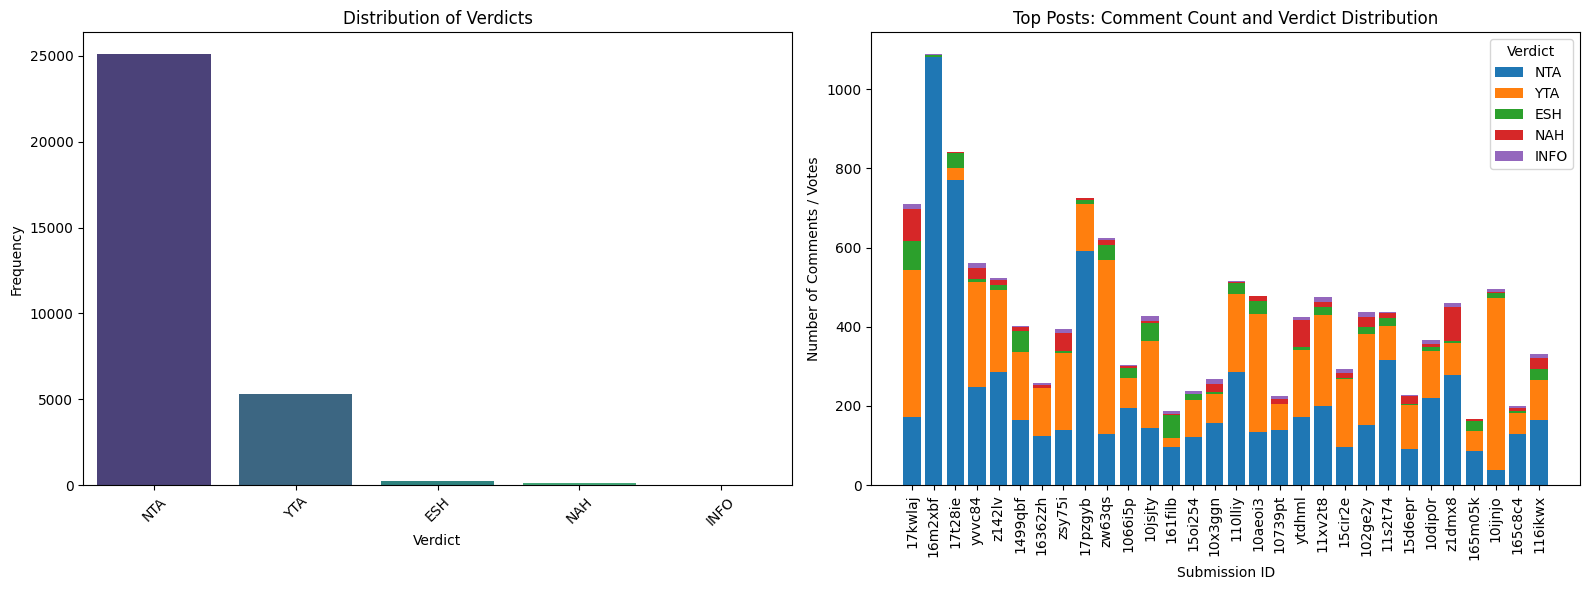
\includegraphics[width=0.45\textwidth]{resources/tendencias.png}
    \caption{Gráfico de tendencias encontradas sobre los datos}
    \label{fig:tendencias}
\end{figure}

Por otro lado, la figura \ref{fig:score-verdict} muestra que los datos no siguen un patrón específico de comportamiento, donde no necesariamente las publicaciones con veredicto YTA son más famosos que los de NTA.

\begin{figure}
    \centering
    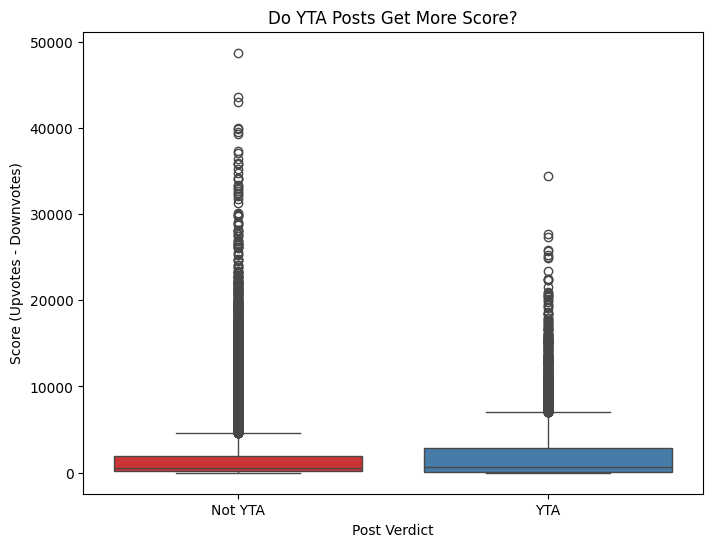
\includegraphics[width=1\linewidth]{resources/score-vs-verdict.png}
    \caption{Puntuación contra el veredicto}
    \label{fig:score-verdict}
\end{figure}

Finalmente, la figura \ref{fig:common-words} muestra algunas de las palabras más utilizadas son palabras muy comunes en la descripción de una historia. La palabra más utilizada es 'said', seguida de 'told' y 'just'. Esto es congruente dado que son verbos o formas de entrelazar una historia. Sin embargo,muchas veces tienen significados semánticos interesantes, donde se habla mucho de las otras personas de una familia "sister", "mom", "family", "wife", etc. Es interesante denotar que en su mayoría son palabras para referirse a personas del género femenino.

\begin{figure}
    \centering
    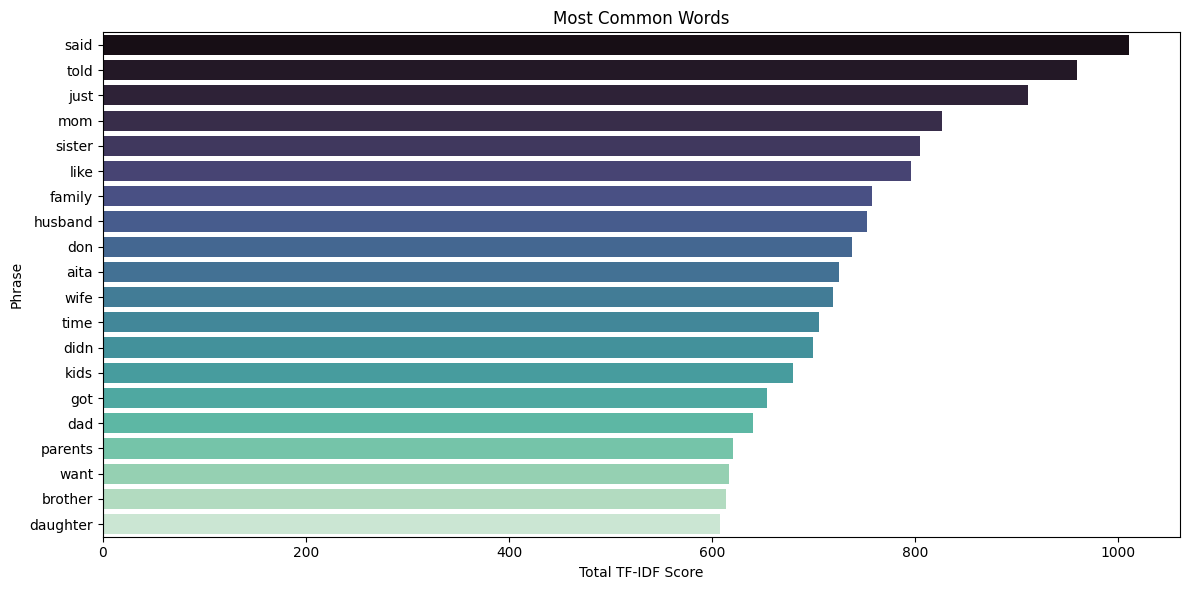
\includegraphics[width=1\linewidth]{resources/common-words.png}
    \hfill
    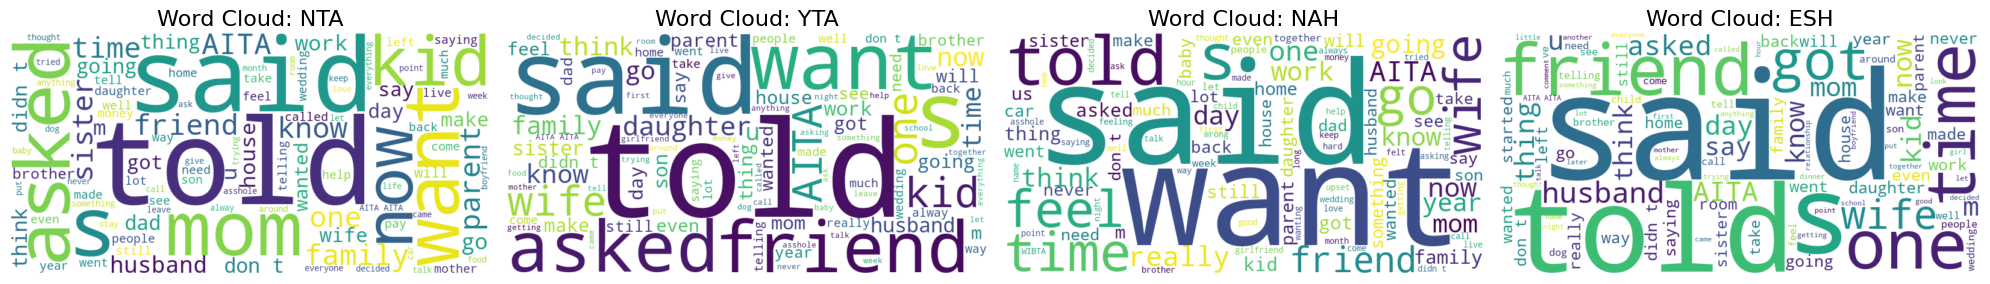
\includegraphics[width=1\linewidth]{resources/word-clouds.png}
    \caption{Palabras más utilizadas, separadas también por clase}
    \label{fig:common-words}
\end{figure}

\subsubsection*{Agrupamiento semántico de temas}

Con el fin de explorar patrones temáticos dentro del corpus, se aplicó un algoritmo de agrupamiento semántico sobre las representaciones vectoriales de las publicaciones, lo cual permitió identificar \textbf{cinco clústeres dominantes}. Cada clúster agrupa publicaciones según vocabulario y contexto compartido, revelando los principales ejes narrativos de los conflictos analizados. Entre los temas más representativos se encuentran: \emph{relaciones de pareja y conflictos matrimoniales}, \emph{dinámicas familiares con hijos}, \emph{disputas con padres y suegros}, \emph{problemas relacionados con mascotas en el hogar}, y \emph{malentendidos en la convivencia}. Esta segmentación temática no solo aporta una visión cualitativa del contenido, sino que también abre la posibilidad de incorporar contexto semántico como variable adicional en futuros modelos de clasificación. Los gráficos \ref{fig:clusters} visualizan los agrupamientos encontrados.


\begin{figure}
    \centering
    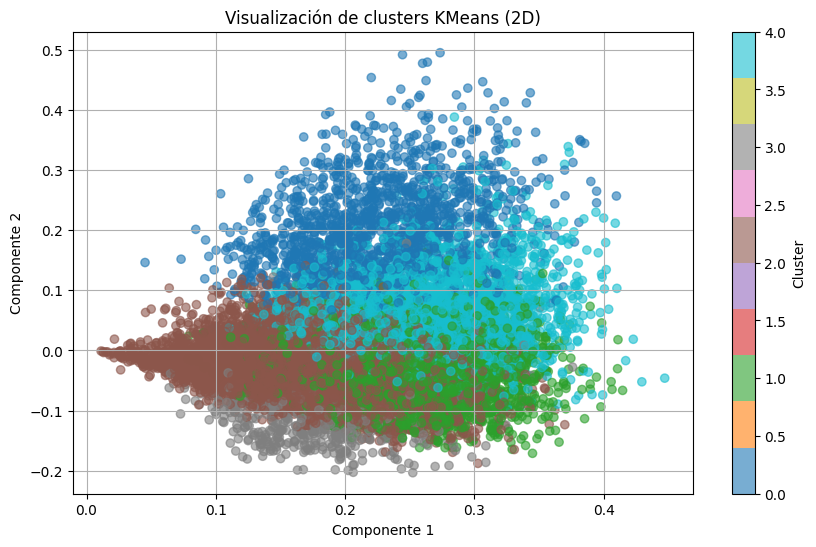
\includegraphics[width=0.45\textwidth]{resources/clusters.png}
    \hfill
    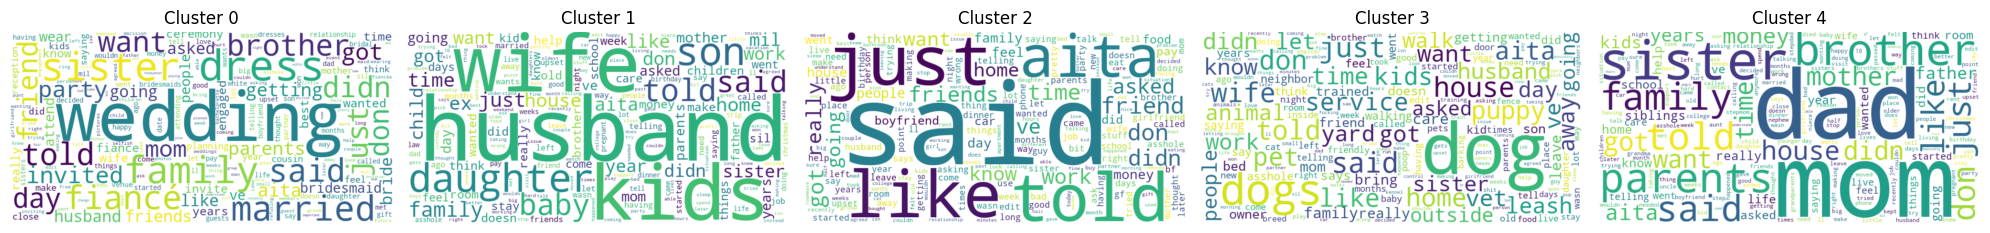
\includegraphics[width=0.45\textwidth]{resources/clusters-2.png}
    \caption{Gráfico de agrupamientos encontradas sobre los datos}
    \label{fig:clusters}
\end{figure}


\subsubsection*{Análisis de sentimiento}

Con el fin de encontrar otros patrones no inherentes a los datos, sino que son observables a través de los mismos, se realizó un análisis de sentimientos (con un modelo pre-entrenado) con el fin de entender si el sentimiento es positivo o negativo dependiendo de la clase. En la figura \ref{fig:sentiment-analysis} se puede ver que en su gran mayoría, los sentimientos que encuentra el modelo son negativos. Lo que tiene mucho sentido. Los usuarios que publican en esta comunidad lo hacen con un propósito de desahogarse, de poder sentir apoyo de otras personas y tener una visión externa de la situación en la que se encuentran.

\begin{figure}
    \centering
    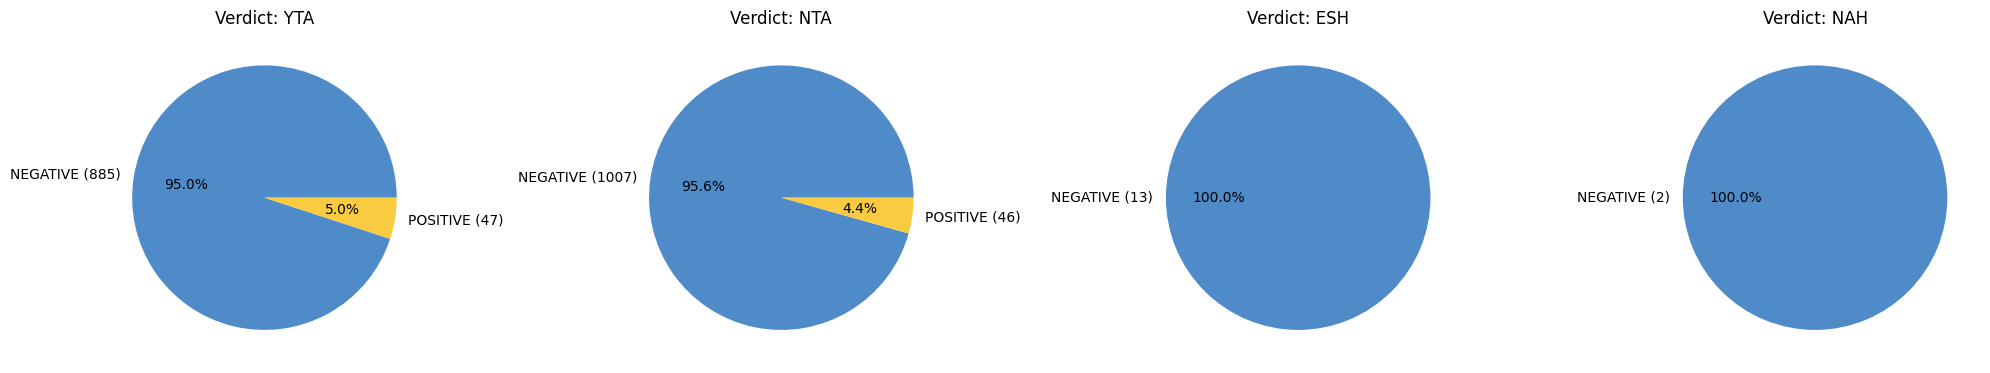
\includegraphics[width=1\linewidth]{resources/sentiment-analysis.png}
    \caption{Gráfico del análisis de sentimiento realizado}
    \label{fig:sentiment-analysis}
\end{figure}

\subsection{Entrenamiento de modelos}

Finalmente dentro de la metodología tenemos el entrenamiento de modelos. Dentro de los objetivos planteados del proyecto estaba la utilización de diferentes modelos de aprendizaje que combinaran diferentes técnicas; tales como el aprendizaje automático clásico, con modelos como la regresión logística, las máquinas de vectores de soporte, entre otros. Y modelos más avanzados, como los grandes modelos de lenguaje (LLMs), o redes recurrentes.

En este orden de ideas, se escogió trabajar los siguientes modelos: 
\begin{itemize}
    \item Clásicos: Regresión logística, Naive Bayes, Máquinas de vectores de soporte.

    Sobre estos modelos se aplicará el aprendizaje tradicional, donde se vectorizan las entradas, generalmente con un vectorizador \verb|Tf-idf|, con el fin de tener un marco de referencia y encontrar patrones interesantes.
    
    \item Aprendizaje profundo: GRU y BERT (y otras variaciones como RoBERTa, XLM-RoBERTa, entre otros).

    Sobre estos modelos se aplicarán dos técnicas. La primera es el aprendizaje desde cero, con el modelo pequeño de GRU, y la segunda es utilizando aprendizaje por transferencia con modelos de la familia BERT. De estos modelos ya se espera un resultado mucho más confiable considerando su naturaleza no-lineal.
    
    \item Grandes modelos de lenguaje: GPT-4o, Llama 3.1.

    Sobre estos modelos no se hará ninguna clase de entrenamiento o fine-tuning. Esto es porque son demasiado grandes. Sin embargo, como son generativos, tienen la capacidad de generar un razonamiento o pensamiento adicional, por lo cual es interesante utilizarlos y ver (con métricas) qué tanto se comparan con respecto a los otros modelos, considerablemente más simples.
    
\end{itemize}

\subsection{Despliegue}

Para el despliegue, el cual será local y no estará disponible en internet, se desarrollará un backend, que tiene la lógica completa de la aplicación, y trabajará con los modelos finales para retornar las predicciones. El frontend, que estará de cara al usuario final, muestra estos resultados permitiendo al usuario ingresar cualquier input, y entender el comportamiento de los modelos a simple vista.



% Experimentos: Presente el diseño experimental, incluyendo escenarios, configuraciones y validaciones.
\section{Experimentos}\label{sec:experimentos}

Todo el código relevante y que se explica en esta sección, se encuentra en el siguiente repositorio de GitHub\footnote{https://github.com/juanyepesp/isis4219-aita-project}.

La estructura del repositorio es la siguiente:

\begin{verbatim}
|- docs
|- src
    |- back
    |- front
    |- notebooks
\end{verbatim}

En el directorio \verb|docs| se encuentra el código fuente de \LaTeX   \ utilizado para este documento. En el directorio \verb|src| está todo el código fuente, o la columna vertebral del proyecto. Dentro de \verb|back| está la lógica que la aplicacion, utilizando todos los modelos entrenados, para hacer las predicciones, dentro del \verb|front| está todo el código para la página web y finalmente dentro de \verb|notebooks| están los cuadernos de Jupyter que se utilizaron para entrenar los modelos, encontrar métricas, hacer fine-tuning, etc. De igual forma, en este último directorio se encuentra el análisis exploratorio de los datos, explicado anteriormente. De igual forma, todos los modelos se prueban con datasets equivalentes. En cuanto a la división de los datos, se asignó un 80\% al conjunto de entrenamiento y un 20\% al conjunto de prueba, reservando además un 20\% del conjunto de entrenamiento como validación interna.

\subsection{Modelos clásicos}

Se evaluaron tres modelos clásicos de aprendizaje automático con el objetivo de establecer líneas base para la tarea planteada. Los modelos implementados fueron: Regresión Logística, Naive Bayes y Máquinas de Vectores de Soporte (SVM). Todos los modelos fueron entrenados y evaluados bajo la misma configuración experimental para garantizar una comparación justa.

\subsubsection{Configuración}
La configuración de entrenamiento fue homogénea para los tres modelos, utilizando una división fija del conjunto de datos entre entrenamiento y prueba. Se empleó una vectorización básica de las entradas (por ejemplo, TF-IDF si se trata de texto), y no se aplicaron técnicas avanzadas de ajuste de hiperparámetros, a excepción de la SVM la cual por su comportamiento se requeria iteraciones adicionales mostradas en la siguiente sección.

Los modelos se implementaron en Python utilizando bibliotecas estándar como scikit-learn, y se evaluaron utilizando métricas clásicas de clasificación.

\subsubsection{Descripción de los modelos}

\begin{itemize}
    \item Regresión Logística (Logistic Regression): Se empleó como un clasificador lineal base por su simplicidad y capacidad de interpretabilidad. Utiliza la función softmax para modelar la probabilidad de pertenencia a una clase.
    \item Naive Bayes: Modelo probabilístico basado en el teorema de Bayes con una fuerte (e irrealista) suposición de independencia entre características. 
    \item SVM (Support Vector Machine): Se utilizó con un kernel RBF (o lineal, si fue el caso), dado que SVM es particularmente eficaz en espacios de alta dimensión. Sin embargo, su rendimiento puede depender fuertemente del ajuste de hiperparámetros.
\end{itemize}

\paragraph{Implementación SVM}
Como se menciono anteriormente,se realizó una implementación exhaustiva de máquinas de vectores de soporte como modelo principal de aprendizaje automático clásico, evaluando diferentes configuraciones de kernels y parámetros para establecer una línea de referencia sólida.

\begin{itemize}
    \item Vectorización especial TF-IDF con eliminación de palabras vacías en inglés, máximo de 20,000 características más relevantes, n-gramas de 1-2 palabras, frecuencia mínima de 2 documentos y máxima de 95\%
    \item Aplicación de submuestreo (downsampling) de la clase mayoritaria NTA para equilibrar el dataset
    \item Validación cruzada de 5 pliegues para evaluar robustez del modelo
\end{itemize}

Se evaluaron tres tipos de kernels fundamentales. Dentro de ellos el Kernel Lineal para establecer línea base con separación lineal, Kernel RBF con parámetro gamma='scale' para capturar patrones no lineales y finalmente Kernel Polinomial para evaluar relaciones polinomiales entre características.

\subsection{Aprendizaje profundo}
Para abordar las limitaciones de los modelos clásicos, especialmente en la comprensión de matices semánticos y el manejo del desbalance de clases, se exploraron arquitecturas de aprendizaje profundo basadas en Transformers, específicamente modelos de la familia BERT (Bidirectional Encoder Representations from Transformers). Estos modelos son preentrenados en grandes corpus de texto y han demostrado un rendimiento sobresaliente en una amplia gama de tareas de Procesamiento del Lenguaje Natural.

\subsubsection{Modelos tipo BERT}
Se diseñaron dos experimentos principales para evaluar diferentes estrategias de aplicación de modelos BERT a la tarea de clasificación de veredictos morales:

\textbf{Configuración Experimental Común:}
\\
Se utilizó el tokenizador específico de cada modelo BERT, como \texttt{AutoTokenizer} de Hugging Face. La longitud máxima de secuencia se fijó en \texttt{MAX\_SEQ\_LEN = 512} tokens, aplicando truncamiento o relleno según fuera necesario. Para el procesamiento por lotes, se empleó un tamaño de lote definido por \texttt{BATCH\_SIZE = 16}.


\textbf{Experimento 1: BERT base congelado (Extracción de Características)}
Se evaluó el rendimiento de un modelo \texttt{bert-base-uncased} preentrenado sin realizar un ajuste fino de sus capas internas. Específicamente, los pesos del cuerpo principal del modelo BERT (capas de atención y embeddings) se mantuvieron congelados. Únicamente se entrenó una nueva capa de clasificación lineal añadida sobre la representación del token \texttt{[CLS]} (o la salida del \textit{pooler}). El objetivo era establecer una línea base del poder representacional de los embeddings preentrenados de BERT para esta tarea.

\textbf{Experimento 2: Fine-tuning completo de modelos BERT}
Se realizó un ajuste fino (\textit{fine-tuning}) completo de tres variantes de modelos BERT: \texttt{bert-base-uncased}, un modelo BERT base estándar no sensible a mayúsculas; \texttt{roberta-base}, una versión optimizada de BERT que modifica aspectos clave del preentrenamiento bajo el enfoque denominado \textit{Robustly optimized BERT approach}; y \texttt{xlm-roberta-base}, un modelo multilingüe basado en RoBERTa, incluido con el objetivo de evaluar si su entrenamiento en múltiples idiomas podría aportar alguna capacidad de generalización útil, a pesar de que la tarea es primordialmente en inglés. En esta configuración, todos los pesos de los modelos, incluyendo las capas de atención y los embeddings, fueron actualizados durante el entrenamiento para adaptarlos específicamente al conjunto de datos y a la tarea de clasificación de veredictos.


\subsubsection{Redes Neuronales Recurrentes (GRU)}
Se implementó una arquitectura de red neuronal recurrente basada en unidades GRU (Gated Recurrent Unit) utilizando TensorFlow/Keras para evaluar la efectividad de enfoques secuenciales alternativos.

\textbf{Configuración Experimental}

La implementación de GRU utilizó una configuración experimental diseñada para aprovechar las características TF-IDF como entrada secuencial. 

Se utilizaron las 200 características TF-IDF más relevantes, seleccionadas por varianza, las cuales fueron transformadas en secuencias de longitud fija para la entrada del modelo. El procesamiento se realizó por lotes con un tamaño de 64 muestras, lo que permitió optimizar tanto el uso de memoria como la velocidad de convergencia del entrenamiento. Para la optimización, se empleó el algoritmo Adam con una tasa de aprendizaje inicial de 0.001. El entrenamiento se llevó a cabo durante un máximo de 20 épocas, implementando una estrategia de early stopping basada en la pérdida de validación, con una paciencia de 5 épocas. Para asegurar un aprendizaje equilibrado, se utilizó el mismo conjunto de datos balanceado mediante submuestreo que se aplicó previamente para los modelos presentados.

\paragraph{Arquitectura del Modelo}
La red neuronal implementada fue una arquitectura secuencial avanzada compuesta por varias capas especializadas. En primer lugar, se utilizó una capa GRU bidireccional con 256 unidades, configurada con "
return\_sequences=True, un dropout del 0.3, dropout recurrente de 0.2 y regularización combinada L1-L2 para controlar el sobreajuste. Posteriormente, se incorporó una capa GRU unidireccional con 128 unidades, esta vez con return\_sequences=False y la misma estrategia de regularización. La red continuó con dos capas densas de 256 y 128 neuronas respectivamente. Entre estas capas densas se añadieron capas dropout con tasas progresivas de 0.4, 0.4 y 0.3 para mejorar la generalización del modelo. Finalmente, la salida se generó a través de una capa softmax, adecuada para la tarea de clasificación multiclase.

\paragraph{Estrategias de Regularización}
Se aplicó dropout en las capas recurrentes y densas con tasas variables. La regularización L1-L2 se utilizó en los kernels de todas las capas GRU y densas. Se incorporó normalización por lotes entre las capas principales. El entrenamiento se controló mediante early stopping, monitoreando la pérdida de validación con una paciencia de 5 épocas. También se implementó una reducción de la tasa de aprendizaje con un factor de 0.5, paciencia de 3 épocas y una tasa mínima de 1e-6. Finalmente, se usó model checkpoint para guardar automáticamente el mejor modelo según la exactitud en la validación.

\subsection{Grandes modelos de lenguaje}

\subsubsection{Llama 3.1 8B Instruct}
Se implementó una evaluación directa del modelo Llama 3.1 8B Instruct utilizando Hugging Face Transformers, aprovechando las capacidades de razonamiento preentrenadas sin entrenamiento adicional específico.

\textbf{Configuración del Modelo}

La implementación utilizó especificaciones técnicas optimizadas. Se empleó el modelo \texttt{meta-llama/Meta-Llama-3.1-8B-Instruct} de Hugging Face. La precisión utilizada fue float16 para optimizar el uso de memoria GPU. La distribución del modelo se realizó mediante device mapping automático, permitiendo una asignación eficiente en el hardware disponible. Además, se configuró \texttt{trust\_remote\_code=True} para permitir la ejecución de código personalizado del modelo.

\textbf{Diseño del Prompt} 

Se desarrolló un prompt estructurado y determinístico. Las instrucciones fueron explícitas, con una definición clara de cada categoría de veredicto. Se estableció una restricción de formato, limitando la salida a cinco etiquetas válidas: YTA, NTA, NAH, ESH e INFO. Asimismo, se utilizó un template consistente para mantener una estructura uniforme y minimizar la variabilidad en las respuestas.

\textbf{Parámetros de Generación} 

La temperatura se fijó en 0.1 para minimizar la aleatoriedad, y la longitud máxima se limitó a 10 tokens nuevos para respuestas concisas. Se activó el muestreo (\texttt{do\_sample=True}) con baja temperatura para asegurar determinismo, y se especificó \texttt{pad\_token\_id=tokenizer.eos\_token\_id} para el manejo correcto de los tokens de relleno.

\textbf{Metodología de Evaluación} 

El procesamiento se realizó en lotes de 100 muestras para optimizar el rendimiento. La extracción de resultados se llevó a cabo con un parser robusto, que incluye un mecanismo de respaldo que asigna la etiqueta "NTA" en caso de fallo. Finalmente, se monitoreó el progreso mediante indicadores cada 1000 muestras procesadas.


\subsubsection{GPT-4o mini}

Se diseñaron dos experimentos complementarios utilizando la API de Azure OpenAI. En primer lugar, se llevó a cabo una evaluación general del modelo, aplicando GPT de OpenAI, específicamente \texttt{gpt-4o-mini} desplegado en Azure, sobre la totalidad del dataset construido, que consta de aproximadamente 30,000 publicaciones. 

\textbf{Prueba Inicial}

Muy parecido al Llama-3.1b, la primera prueba del experimento consistió en aplicar el modelo \texttt{gpt-4o-mini} (desplegado en Azure OpenAI) sobre el conjunto completo de publicaciones procesadas. Se utilizó un \texttt{prompt} de sistema diseñado para instruir al modelo a actuar como clasificador de veredictos. La temperatura de generación se fijó inicialmente en 0.8 para esta evaluación. Durante la ejecución del modelo, se detectaron múltiples entradas que generaban errores por restricciones asociadas a la cuenta educativa utilizada (filtros de moderación del servicio). Estas entradas fueron registradas y almacenadas por separado en un nuevo dataset con etiquetas \texttt{ERROR}, lo cual permitió continuar la evaluación del modelo sobre las muestras válidas sin comprometer la integridad de los resultados.

\textbf{Análisis del impacto de la temperatura}

Con el fin de analizar el efecto del parámetro de temperatura en el rendimiento del modelo \texttt{gpt-4o-mini}, se diseñó un segundo experimento a partir de un subconjunto del conjunto de datos original. Se seleccionó aleatoriamente un 35\% del dataset inicial y se aplicó una segunda limpieza para remover aquellas entradas que habían generado errores en la primera fase, típicamente debido a restricciones de moderación impuestas por la cuenta educativa de Azure.

El nuevo conjunto reducido y depurado fue utilizado para realizar inferencias con cuatro configuraciones distintas de temperatura: \texttt{0.0}, \texttt{0.4}, \texttt{0.8} y \texttt{1.0}. El propósito de este experimento fue evaluar cómo varía la precisión del modelo en función del nivel de aleatoriedad introducido en las respuestas generadas, donde el contexto puede ser interpretado de múltiples formas. 

% Resultados y Discusión: Muestre los resultados obtenidos, compárelos con otros trabajos o enfoques base, y discuta su significado.
\section{Resultados y Discusión}

\subsection{Modelos Clásicos}

Los modelos fueron evaluados utilizando métricas estándar para tareas de clasificación multiclase: \textit{accuracy}, \textit{precision}, \textit{recall} y \textit{F1-score}. Se reportan tanto los promedios \textit{macro} como los promedios ponderados (\textit{weighted}), así como las métricas específicas por clase.

Dado que algunas clases tienen considerablemente menos instancias que otras, el promedio ponderado proporciona una visión más ajustada al desequilibrio de clases, mientras que el promedio macro permite observar si los modelos logran generalizar más allá de las clases dominantes.

A continuación se presenta una cuadro resumen con los resultados de cada modelo:

\begin{table}[H]
\centering
\caption{Comparación de modelos clásicos en métricas globales.}
\begin{tabular}{lccc}
\toprule
\textbf{Modelo} & \textbf{Accuracy} & \textbf{Macro F1} & \textbf{Weighted F1} \\
\midrule
Naive Bayes            & 0.55 & 0.21 & 0.50 \\
Regresión Logística    & 0.60 & 0.25 & 0.59 \\
SVM                    & 0.61 & 0.25 & 0.60 \\
\bottomrule
\end{tabular}
\end{table}

Las métricas por clase revelan que los modelos tienden a enfocarse casi exclusivamente en las clases mayoritarias (NTA y YTA), con un desempeño prácticamente nulo en las clases minoritarias (ESH, INFO, NAH). Esto se ve reflejado en que tanto la precisión como el \textit{recall} para estas clases son cero en todos los modelos. El modelo Naive Bayes presenta la mayor caída en \textit{F1-score} ponderado, mientras que SVM logra un leve mejor desempeño general.

\subsection{Aprendizaje Profundo}

\subsubsection{Modelos tipo BERT}

Los experimentos con modelos basados en la arquitectura Transformer, específicamente variantes de BERT, buscaron superar las limitaciones de los modelos clásicos mediante la captura de relaciones semánticas complejas y un mejor manejo del desbalance de clases a través de funciones de pérdida especializadas como \texttt{WeightedFocalLoss}. La evaluación de estos modelos se centró en su capacidad para generalizar a partir de los datos de entrenamiento y clasificar correctamente los veredictos morales, prestando especial atención a las métricas F1-score macro y ponderado debido al desequilibrio inherente en las clases.

A continuación, se presenta una cuadro comparativa con las métricas globales obtenidas en el conjunto de prueba para los diferentes modelos BERT entrenados y sus configuraciones:

\begin{table}[H]
\centering
\caption{Comparación de modelos tipo BERT en métricas globales (conjunto de prueba).}
\label{tab:bert_results}
\begin{tabular}{@{}lccc@{}}
\toprule
\textbf{Modelo y Configuración} & \textbf{Accuracy} & \textbf{Macro F1} & \textbf{Weighted F1} \\
\midrule
\texttt{base-uncased} (Frozen) & 0.46 & 0.18 & 0.50 \\
\texttt{base-uncased} & 0.74 & 0.25 & 0.75 \\
\texttt{roberta-base}  & 0.72 & 0.26 & 0.74 \\

\bottomrule
\end{tabular}
\end{table}


Para un análisis más especifico, la cuadro \ref{tab:bert_f1_per_class} muestra los F1-scores por cada clase para los modelos BERT evaluados.

\begin{table}[H]
\centering
\caption{F1-score por clase para modelos tipo BERT (conjunto de prueba).}
\label{tab:bert_f1_per_class}
\begin{tabular}{@{}lccccc@{}}
\toprule
\textbf{Modelo} & \textbf{NTA} & \textbf{YTA} & \textbf{ESH} & \textbf{NAH} & \textbf{INFO} \\
\midrule
\texttt{base-uncased} (F) & 0.53 & 0.38 & 0.00 & 0.00 & 0.00 \\
\texttt{base-uncased} & 0.84 & 0.39 & 0.00 & 0.00 & 0.00 \\
\texttt{roberta-base}  & 0.82 & 0.46 & 0.00 & 0.00 & 0.00 \\

\bottomrule
\end{tabular}
\end{table}

\subsubsection{Análisis de Resultados de Modelos BERT}

El primer enfoque utilizó \texttt{bert-base-uncased} con sus capas principales congeladas, entrenando únicamente una capa de clasificación superior, funcionando como línea base. Este modelo alcanzó un F1-score macro de 0.18 y una exactitud de 0.46 (ver cuadro \ref{tab:bert_results}). El desglose por clase (cuadro \ref{tab:bert_f1_per_class}) muestra un F1-score de 0.53 para la clase mayoritaria \texttt{NTA} y 0.38 para \texttt{YTA}, pero un rendimiento nulo (0.00) para las clases minoritarias \texttt{ESH}, \texttt{NAH} e \texttt{INFO}. Aunque el F1-score macro global es modesto, indica que los embeddings preentrenados capturan información semántica relevante, aunque insuficiente para las clases menos representadas sin un ajuste fino.

El ajuste fino completo de los modelos BERT produjo mejoras significativas. El modelo \texttt{bert-base-uncased} con fine-tuning logró un F1-score macro de 0.25 y una exactitud del 74\% (cuadro \ref{tab:bert_results}). A nivel de clase (cuadro \ref{tab:bert_f1_per_class}), el F1-score para \texttt{NTA} aumentó a 0.84 y para \texttt{YTA} a 0.39. Aunque esto representa un aumento considerable, las clases minoritarias continuaron con un F1-score de 0.00, demostrando la persistencia del desafío del desbalance. De manera similar, el modelo \texttt{roberta-base} con fine-tuning alcanzó un F1-score macro de 0.26 y una exactitud del 72\%. Este modelo mostró el F1-score macro más alto entre los evaluados, con F1-scores por clase de 0.82 para \texttt{NTA} y un notable 0.46 para \texttt{YTA}, el mejor para esta segunda clase mayoritaria. No obstante, al igual que con \texttt{bert-base-uncased}, las clases \texttt{ESH}, \texttt{NAH} e \texttt{INFO} no fueron correctamente identificadas (F1-score de 0.00). Los resultados para \texttt{xlm-roberta-base} aún están pendientes (TBD).

A pesar de las mejoras con el fine-tuning, los F1-scores macro relativamente bajos (0.25-0.26) y el rendimiento nulo en las clases minoritarias (cuadro \ref{tab:bert_f1_per_class}) subrayan que, aunque los modelos son significativamente mejores que los modelos clásicos y el BERT congelado, el principal desafío sigue siendo la correcta clasificación de las clases con pocas instancias.


\end{enumerate}


En conjunto, los modelos basados en la arquitectura BERT demostraron una clara superioridad sobre los enfoques clásicos. El \textit{fine-tuning} es esencial para adaptar estos modelos preentrenados a las particularidades del lenguaje y la estructura de las publicaciones del subreddit.
La función de pérdida \texttt{WeightedFocalLoss} fue un componente crucial para mitigar parcialmente el impacto del severo desbalance de clases. Sin embargo, como se evidencia en la cuadro \ref{tab:bert_f1_per_class}, las clases mayoritarias \texttt{NTA} y \texttt{YTA} son consistentemente mejor clasificadas, mientras que las clases \texttt{ESH}, \texttt{NAH}, e \texttt{INFO} permanecen como un desafío significativo, con F1-scores nulos en todos los modelos BERT evaluados hasta ahora.
Las limitaciones observadas sugieren que, además de la arquitectura del modelo y la función de pérdida, podrían explorarse estrategias adicionales como técnicas de aumento de datos específicas para texto en clases minoritarias, o métodos de muestreo más sofisticados durante el entrenamiento. 
%La incorporación de características numéricas (Experimento 3) también representa una vía prometedora para enriquecer la información disponible para el modelo.

\subsubsection{Redes Neuronales Recurrentes (GRU)}

Como enfoque alternativo al aprendizaje profundo basado en transformers, se implementó y evaluó una arquitectura de red neuronal recurrente utilizando unidades GRU bidireccionales. Este modelo fue diseñado para capturar dependencias secuenciales en las representaciones TF-IDF y explorar si las arquitecturas recurrentes pueden ofrecer ventajas en términos de eficiencia computacional manteniendo un rendimiento competitivo.

\paragraph{Resultados del Modelo GRU}

El modelo GRU entrenado durante 20 épocas con early stopping alcanzó los siguientes resultados en el conjunto de prueba:

\begin{table}[H]
\centering
\caption{Métricas globales del modelo GRU.}
\begin{tabular}{lccc}
\toprule
\textbf{Métrica} & \textbf{Valor} & \textbf{Pérdida} & \textbf{Accuracy} \\
\midrule
Precision (weighted) & 0.4833 & 0.9949 & 0.5015 \\
Recall (weighted) & 0.5015 & - & - \\
F1-Score (weighted) & 0.4499 & - & - \\
F1-Score (macro) & 0.19 & - & - \\
\bottomrule
\end{tabular}
\end{table}

El análisis por clase revela un patrón similar al observado en otros modelos, con una concentración del rendimiento en las clases mayoritarias:

\begin{table}[H]
\centering
\caption{Métricas por clase del modelo GRU.}
\begin{tabular}{lcccc}
\toprule
\textbf{Clase} & \textbf{Precision} & \textbf{Recall} & \textbf{F1-Score} & \textbf{Support} \\
\midrule
ESH & 0.00 & 0.00 & 0.00 & 53 \\
INFO & 0.00 & 0.00 & 0.00 & 9 \\
NAH & 0.00 & 0.00 & 0.00 & 34 \\
NTA & 0.50 & 0.80 & 0.62 & 1162 \\
YTA & 0.51 & 0.23 & 0.31 & 1105 \\
\bottomrule
\end{tabular}
\end{table}

\paragraph{Análisis del Rendimiento GRU}

El modelo GRU mostró un rendimiento del 50.15\% de accuracy, situándose en un nivel intermedio entre los modelos clásicos y los más avanzados basados en transformers. En cuanto a las clases mayoritarias, el modelo alcanzó un F1-score de 0.62 para NTA y 0.31 para YTA, lo que indica una capacidad moderada para distinguir entre las dos clases principales. Sin embargo, al igual que otros modelos evaluados, no logró identificar correctamente instancias de las clases minoritarias ESH, INFO y NAH, obteniendo F1-scores de 0.00. En términos de eficiencia computacional, debido a un tiempo de entrenamiento significativamente menor que los modelos transformer, el GRU representa una alternativa computacionalmente más eficiente.

\paragraph{Comparación con Otros Enfoques}

El modelo GRU se posiciona como una opción intermedia en términos de rendimiento y complejidad computacional. Mientras que no alcanza la precisión de los modelos BERT con fine-tuning, supera a los modelos clásicos y ofrece ventajas en términos de recursos computacionales requeridos y tiempo de entrenamiento.

La convergencia del modelo fue estable, con el early stopping activándose efectivamente para prevenir sobreajuste. Las técnicas de regularización implementadas (dropout, regularización L1-L2, normalización por lotes) contribuyeron a mantener un balance entre capacidad de aprendizaje y generalización.

\subsection{Grandes modelos de lenguaje}

\subsubsection{Llama 3.1 8B Instruct}

El modelo Llama 3.1 8B Instruct fue evaluado mediante inferencia directa sin entrenamiento adicional, utilizando un prompt estructurado para la clasificación de veredictos morales. Esta evaluación permite determinar las capacidades inherentes del modelo preentrenado para comprender y clasificar dilemas éticos complejos.

\paragraph{Resultados Generales}

El modelo fue evaluado sobre el conjunto completo de datos (30,303 publicaciones) y alcanzó un accuracy general del 47.12%. Los resultados detallados se presentan a continuación:

\begin{table}[H]
\centering
\caption{Métricas globales del modelo Llama 3.1 8B Instruct.}
\begin{tabular}{lccc}
\toprule
\textbf{Promedio} & \textbf{Precision} & \textbf{Recall} & \textbf{F1-Score} \\
\midrule
Macro & 0.2194 & 0.2347 & 0.1965 \\
Weighted & 0.7123 & 0.4712 & 0.5634 \\
\bottomrule
\end{tabular}
\end{table}

\paragraph{Análisis por Clase}

El rendimiento por clase muestra patrones interesantes que difieren de los modelos previamente evaluados:

\begin{table}[H]
\centering
\caption{Métricas detalladas por clase - Llama 3.1 8B Instruct.}
\begin{tabular}{lcccc}
\toprule
\textbf{Clase} & \textbf{Precision} & \textbf{Recall} & \textbf{F1-Score} & \textbf{Support} \\
\midrule
YTA & 0.2456 & 0.5234 & 0.3341 & 5,389 \\
NTA & 0.8156 & 0.4567 & 0.5887 & 24,467 \\
NAH & 0.0156 & 0.0633 & 0.0252 & 158 \\
ESH & 0.0167 & 0.0944 & 0.0282 & 233 \\
INFO & 0.0034 & 0.0357 & 0.0063 & 56 \\
\bottomrule
\end{tabular}
\end{table}

\paragraph{Características Distintivas del Rendimiento}

Los resultados de Llama 3.1 revelan varios aspectos notables:

\begin{itemize}
    \item A diferencia de los modelos anteriores, Llama 3.1 logró identificar algunas instancias de las clases minoritarias (NAH, ESH, INFO), aunque con precision muy baja
    \item El modelo mostró un recall relativamente alto para YTA (0.5234) comparado con NTA (0.4567), sugiriendo una menor tendencia a favorecer exclusivamente la clase mayoritaria
    \item Mantuvo una alta precisión (0.8156) para la clase NTA, indicando que cuando predice esta categoría, generalmente es correcta
    \item Se registraron 789 entradas con errores durante la inferencia, representando el 2.6\% del conjunto total
\end{itemize}

\paragraph{Matriz de Confusión}

El análisis de la matriz de confusión revela los patrones de error del modelo:

\begin{center}
\small
\begin{tabular}{c|ccccc}
\textbf{Real/Pred.} & \textbf{YTA} & \textbf{NTA} & \textbf{NAH} & \textbf{ESH} & \textbf{INFO} \\
\hline
\textbf{YTA} & 2,821 & 1,894 & 267 & 298 & 109 \\
\textbf{NTA} & 9,234 & 11,167 & 512 & 2,987 & 567 \\
\textbf{NAH} & 45 & 67 & 10 & 26 & 10 \\
\textbf{ESH} & 156 & 54 & 8 & 22 & 3 \\
\textbf{INFO} & 18 & 24 & 6 & 6 & 2 \\
\end{tabular}
\end{center}

\paragraph{Discusión del Rendimiento}

El modelo Llama 3.1 8B Instruct demostró capacidades interesantes para la comprensión de contextos morales sin entrenamiento específico. Aunque su accuracy general (47.12\%) es inferior a los modelos fine-tuned, su capacidad para detectar clases minoritarias y mantener un balance relativo entre YTA y NTA sugiere una comprensión más matizada de los diferentes tipos de veredictos morales.

La evaluación sin fine-tuning proporciona insights valiosos sobre las capacidades emergentes de los LLMs en tareas de razonamiento moral, estableciendo un baseline para futuras investigaciones que podrían explorar técnicas de few-shot learning o prompt engineering más sofisticadas.

\subsubsection{GPT-4o-mini}

El modelo \texttt{gpt-4o-mini}, evaluado sobre la totalidad del conjunto de datos (30.303 publicaciones) con una temperatura de 0.8, alcanzó un \texttt{accuracy} general de 59.80\% y un \texttt{F1-score macro} de 0.2468. La clase con mejor desempeño fue \texttt{NTA} con un F1 de 0.7227, seguida de \texttt{YTA} con 0.4228, mientras que las clases \texttt{NAH}, \texttt{ESH} e \texttt{INFO} mostraron resultados significativamente inferiores. 

A continuación, se presenta el reporte de rendimiento del modelo:

\begin{center}
\small
\begin{tabular}{c|ccccc}
\textbf{Real/Pred.} & \textbf{YTA} & \textbf{NTA} & \textbf{NAH} & \textbf{ESH} & \textbf{INFO} \\
\hline
\textbf{YTA} & 3,544 & 1,035 & 154 & 496 & 160 \\
\textbf{NTA} & 7,654 & 14,516 & 480 & 1,312 & 505 \\
\textbf{NAH} & 30 & 80 & 16 & 13 & 19 \\
\textbf{ESH} & 137 & 45 & 7 & 41 & 3 \\
\textbf{INFO} & 11 & 28 & 10 & 3 & 4 \\
\end{tabular}
\end{center}


Durante la ejecución, 449 entradas fueron rechazadas por el filtro de moderación de contenido de Azure OpenAI y fueron excluidas del cálculo de métricas. Estos casos se registraron por separado en el archivo \texttt{aita\_errores\_filtrados.csv} para posteriores análisis y limpieza.

Este experimento evidenció que, aunque el modelo generaliza bien para las clases predominantes (\texttt{YTA}, \texttt{NTA}), su rendimiento disminuye notablemente en clases minoritarias, lo cual refleja tanto el desbalance del dataset como posibles limitaciones contextuales del modelo bajo temperatura moderadamente creativa (0.8).

\textbf{Comparación por temperatura}

En el segundo experimento se evaluó el efecto de la temperatura sobre el rendimiento del modelo, utilizando un subconjunto del 35\% del dataset original (10.615 entradas válidas tras limpieza). La siguiente cuadro resume los resultados obtenidos para cuatro configuraciones distintas de temperatura:

\begin{table}[h]
\centering
\caption{Rendimiento del modelo GPT-4o-mini con distintas temperaturas (subset del 35\%)}
\begin{tabular}{|c|c|c|}
\hline
\textbf{Temperatura} & \textbf{Accuracy (\%)} & \textbf{F1-score Macro} \\
\hline
0.0 & 62.21 & 0.2616 \\
0.4 & 61.36 & 0.2577 \\
0.8 & 60.64 & 0.2535 \\
1.0 & 61.31 & 0.2522 \\
\hline
\end{tabular}
\label{tab:temperatura}
\end{table}

Los resultados muestran una ligera mejora en el desempeño general a temperaturas más bajas. En particular, el mejor rendimiento se obtuvo con temperatura 0.0, alcanzando una precisión del 62.21\% y un F1-score macro de 0.2616. A medida que se incrementa la temperatura, el modelo se vuelve más variable en sus respuestas, lo cual parece afectar negativamente la consistencia en una tarea de clasificación moral con clases desbalanceadas. No se registraron errores de moderación en esta fase pues anteriormente se limpio el dataset con los resultados obtenidos del primer experimento, lo cual permitió una comparación limpia entre configuraciones.

Este análisis sugiere que, para tareas de clasificación moral automática como esta, donde se espera consistencia y determinismo, es preferible utilizar configuraciones de temperatura más bajas.

\subsection{Comparación General de Modelos}

La evaluación comprehensiva de diferentes paradigmas de aprendizaje automático para la clasificación de veredictos morales revela patrones interesantes y desafíos persistentes en esta tarea específica.

\begin{table}[H]
\centering
\caption{Comparación global de todos los modelos evaluados.}
\begin{tabular}{lccc}
\toprule
\textbf{Modelo} & \textbf{Accuracy} & \textbf{Macro F1} & \textbf{Weighted F1} \\
\midrule
SVM (mejor clásico) & 0.61 & 0.25 & 0.60 \\
GRU & 0.50 & 0.19 & 0.45 \\
BERT (fine-tuned) & 0.74 & 0.25 & 0.75 \\
RoBERTa (fine-tuned) & 0.72 & 0.26 & 0.74 \\
Llama 3.1 8B & 0.47 & 0.20 & 0.56 \\
GPT-4o mini (T=0.0) & 0.62 & 0.26 & - \\
\bottomrule
\end{tabular}
\end{table}

Los resultados demuestran que los modelos basados en transformer con fine-tuning (BERT, RoBERTa) logran el mejor rendimiento general, seguidos por los modelos clásicos optimizados (SVM) y los LLMs sin entrenamiento específico. El modelo GRU, aunque eficiente computacionalmente, mostró el rendimiento más modesto entre los enfoques de aprendizaje profundo evaluados.

\subsection{Despliegue}

En cuanto al despliegue de la solución, cuyo código fuente se encuentra en el repositorio anteriormente descrito, la interfaz de usuario se ubica en la figura \ref{fig:despliegue}, donde se ubica un capo de texto donde el usuario ingresa el texto, y luego de hacer clic en el botón de predicción se muestran los resultados de los modelos más relevantes, donde se expone la categoría encontrada y el razonamiento si aplica, junto con una gráfica que muestra los votos de cada categoría.

\begin{figure}
    \centering
    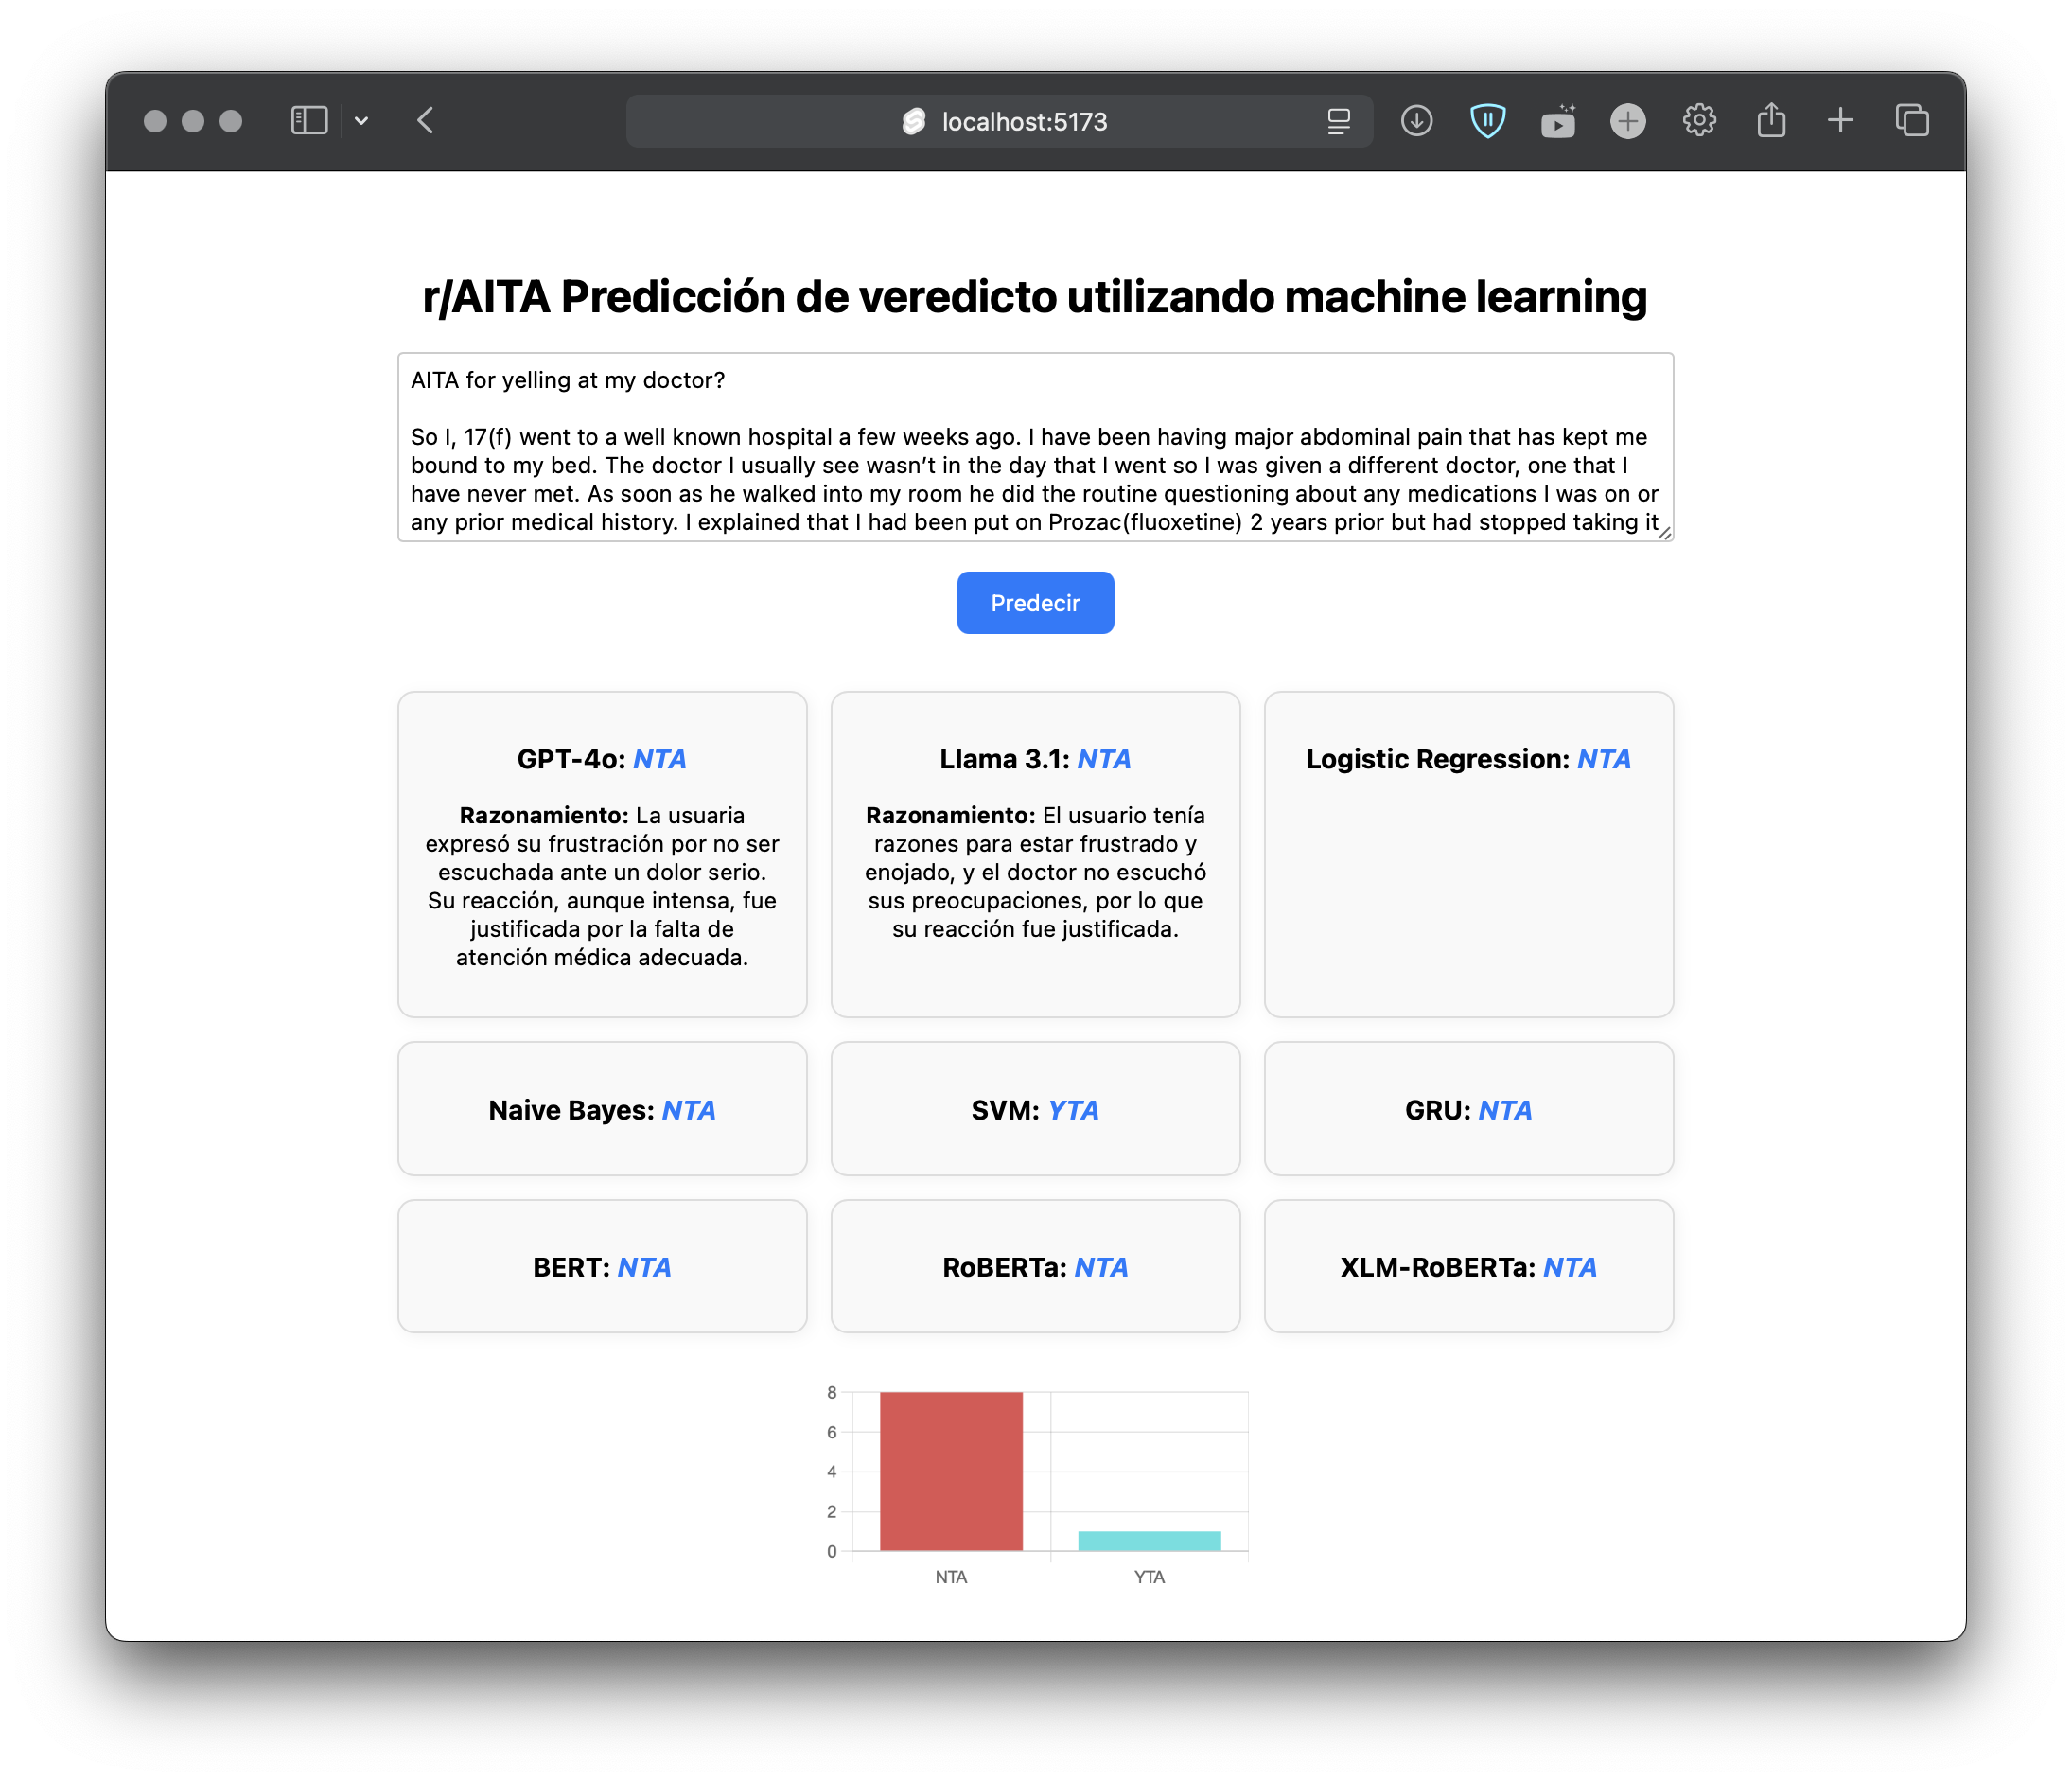
\includegraphics[width=1\linewidth]{resources/despliegue.png}
    \caption{Interfaz de usuario}
    \label{fig:despliegue}
\end{figure}


\subsubsection{Resumen Comparativo de Resultados por Dimensión Analítica}

En la cuadro \ref{tab:comparativo_dimensiones} al final del documento, se presenta una cuadro resumen que compara el desempeño de los diferentes enfoques evaluados, agrupando los modelos por tipo y resaltando sus fortalezas y debilidades en distintas dimensiones clave.



\section{Conclusiones}

En cuanto a los tres modelos clásicos de aprendizaje automático, con el objetivo de establecer una línea base de rendimiento para una tarea compleja de clasificación multiclase. A pesar de sus limitaciones, estos modelos permiten comprender los desafíos fundamentales del problema y brindan un marco de comparación necesario para justificar el uso de enfoques más avanzados.

Los resultados de los modelos clásicos mostraron un rendimiento limitado en términos de precisión, \textit{recall} y \textit{F1-score}, particularmente en las clases minoritarias. Esto evidencia que no son capaces de capturar la complejidad semántica y los matices del conjunto de datos, lo cual era en gran medida esperado debido a la naturaleza del problema.

Por otro lado, las técnicas de aprendizaje profundo, específicamente los modelos basados en la arquitectura Transformer (BERT), demostraron una capacidad superior, en comparación con GRU para aprovechar la estructura y el contexto de los datos textuales. Los experimentos con \texttt{bert-base-uncased} y \texttt{roberta-base} mediante fine-tuning completo mostraron una mejora sustancial sobre los modelos clásicos y la configuración de BERT con capas congeladas. \texttt{roberta-base} (fine-tuned) alcanzó el F1-score macro más alto entre estos modelos, con un 0.26, y un accuracy del 72\%.

Los resultados obtenidos en los dos experimentos realizados para los grandes modelos de lenguaje, como \texttt{gpt-4o-mini}, revelan que es capaz de replicar parcialmente los juicios morales. El modelo mostró un rendimiento aceptable en las clases mayoritarias (\texttt{NTA} y \texttt{YTA}), pero una capacidad significativamente menor para identificar correctamente veredictos menos frecuentes como \texttt{NAH}, \texttt{ESH} e \texttt{INFO}.Por otra parte, el modelo LLaMA 3.1 8B Instruct demostró un rendimiento competitivo. A diferencia de otros modelos evaluados, mostró cierta capacidad para reconocer clases minoritarias como ESH, NAH e INFO, aunque con precisión aún limitada. Esto sugiere que estos LLMs tienen potencial como herramientas de clasificación sin entrenamiento adicional, y que su rendimiento puede mejorar si se les hace un fine-tuning para que sean específicos a estos casos de clasificación.



\bibliographystyle{IEEEtran}
\bibliography{references}

\clearpage
\begin{landscape}
\begin{table}[H]
\centering
\caption{Resumen comparativo de resultados por tipo de modelo.}
\label{tab:comparativo_dimensiones}
\begin{tabular}{|p{4.5cm}|p{4.5cm}|p{6cm}|p{6cm}|}
\hline
\textbf{Criterio} & \textbf{Modelos Clásicos} & \textbf{Aprendizaje Profundo (GRU / BERT)} & \textbf{LLMs sin Fine-Tuning (LLaMA / GPT-4o)} \\
\hline
\textbf{Exactitud General (\textit{Accuracy})} & 0.55--0.61 (SVM mejor) & GRU: 0.50\newline BERT: hasta 0.74 (fine-tuned) & LLaMA: 0.47\newline GPT-4o: hasta 0.62 (T=0.0) \\
\hline
\textbf{F1-Score Macro} & 0.21--0.25 & GRU: 0.19\newline BERT: 0.25--0.26 & LLaMA: 0.20\newline GPT-4o: hasta 0.26 (T=0.0) \\
\hline
\textbf{F1-Score Weighted} & 0.50--0.60 & GRU: 0.45\newline BERT: hasta 0.75 & LLaMA: 0.56\newline GPT-4o: -- \\
\hline
\textbf{Detección de Clases Minoritarias} & Nula (F1 = 0.00) & Nula en todos los casos (F1 = 0.00) & Parcial, aunque con bajo desempeño (F1 < 0.03) \\
\hline
\textbf{Balance entre NTA y YTA} & Fuerte sesgo a clase NTA & Mejorado con fine-tuning (mayor precisión en ambas) & GPT-4o logra balance aceptable; LLaMA tiene mejor recall en YTA que NTA \\
\hline
\textbf{Robustez ante desbalance de clases} & Muy limitada & Mejor con \texttt{WeightedFocalLoss}, pero aún insuficiente & Parcialmente robustos, sin necesidad de técnicas adicionales \\
\hline
\textbf{Ventajas Computacionales} & Alta eficiencia y rapidez & BERT más costoso, GRU más liviano y rápido & Requieren alta capacidad computacional y recursos externos \\
\hline
\end{tabular}
\end{table}
\end{landscape}


\end{document}
